%% 02.tex
\documentclass[platex,dvipdfmx,draft]{jsreport}

\usepackage{graphicx}
\graphicspath{{./images}{../images}}
\usepackage{pdfpages}
\usepackage{tikz}
\usepackage{xcolor}
\definecolor{UD_GREEN}{HTML}{03af7a}
\usepackage{bm}
\usepackage[left=30truemm]{geometry}
\usepackage{amsmath,amssymb}
\numberwithin{equation}{section}

\begin{document}

\chapter{原理}
\section{Maxwell方程式}
フォトニック結晶における電磁波の振る舞いは、Maxwell方程式によって記述される。Maxwell方程式は以下のように表される。
\begin{align}
  \nabla \times \bm{E} &= -\frac{\partial \bm{B}}{\partial t} \\
  \nabla \times \bm{H} &= \bm{j} + \frac{\partial \bm{D}}{\partial t} \\
  \nabla \cdot \bm{D} &= \rho \\
  \nabla \cdot \bm{B} &= 0
\end{align}

今回は、自由電荷や電流のない均一な誘電物質の混合誘電媒体を考えるため、$\rho = 0$、$\bm{j} = 0$となる。また、低損失の誘電体において、$\bm{D} = \epsilon(r) \bm{E}(\bm{r})$、透過率$\mu = 1$とみなすことで$\bm{B}(\bm{r}) = \mu \bm{H}(\bm{r}) = \bm{H}(\bm{r})$となる。

一般に、$\bm{E}$と$\bm{H}$は時間空間における複雑な関数であるが、Maxwell方程式は線形であることから、$\bm{E}$と$\bm{H}$を時間と空間の関数に分離することができる。すなわち、$\bm{E}(\bm{r},t) = \bm{E}(\bm{r}) e^{-i\omega t}$、$\bm{H}(\bm{r},t) = \bm{H}(\bm{r}) e^{-i\omega t}$とすることができ、Maxwell方程式は以下のように表される。
\begin{align}
  \nabla \cdot \bm{H}(\bm{r}) &= 0 \\
  \nabla \cdot \bm{D}(\bm{r}) &= 0 \\
  \label{eq:curlE}
  \nabla \times \bm{E}(\bm{r}) &= - \frac{i \omega}{c} \bm{H}(\bm{r}) \\
  \label{eq:curlH}
  \nabla \times \bm{H} (\bm{r}) &= \frac{i \omega}{c} \epsilon(\bm{r}) \bm{E}(\bm{r})
\end{align}

式(\ref{eq:curlE})と式(\ref{eq:curlH})より$\bm{E}(\bm{r})$を消去して、$\bm{H}(\bm{r})$についての式に整理すると以下のマスター方程式を得ることができる。
\begin{align}
  \label{eq:master}
  \nabla \times \left( \frac{1}{\epsilon (\bm{e})} \nabla \times \bm{H}(\bm{r}) \right) = \left( \frac{\omega}{c} \right)^2 \bm{H}(\bm{r}) 
\end{align}

式(\ref{eq:master})を固有値問題とするために、左辺の$\bm{H}(\bm{r})$に作用する演算子$\hat{\Theta}$を定義する。演算子$\hat{\Theta}$は回転を取り、$\epsilon(\bm{r})$で割って再度回転を取る微分演算子である。

次に、2つのベクトル場$\bm{F}$と$\bm{G}$について内積を以下のように定義する。
\begin{align}
  (\bm{F}, \bm{G}) = \int d\bm{r} \bm{F}^*(\bm{r}) \cdot \bm{G}(\bm{r})
\end{align}

このとき、演算子$\hat{\Theta}$は、任意のベクトル場$\bm{F}, \bm{G}$に対して次の内積関係が成立する。
\begin{align}
  \label{eq:inner}
  (\bm{F}, \hat{\Theta} \bm{G}) = (\hat{\Theta} \bm{F}, \bm{G})
\end{align}

式(\ref{eq:inner})は、演算子$\hat{\Theta}$がエルミート演算子であることを示しており、これはマスター方程式(\ref{eq:master})を解くときに得られる固有値が実数になりうことや固有値が異なる固有関数は互いに直行することなど、量子力学のシュレディンガー方程式と類似している。

マスター方程式(\ref{eq:master})にBlochの定理を適用すると、マスター方程式の解は次のように表される。
\begin{align}
  \bm{H}_{\bm{k}}(\bm{r}) = e^{i \bm{k} \cdot \bm{r}} \bm{u}_{\bm{k}}(\bm{r}) = e^{i \bm{k} \cdot \bm{r}} \bm{u}_{\bm{k}}(\bm{r + R})
\end{align}
ここで、$\bm{k}$はブロッホ波ベクトル、$\bm{R}$は格子ベクトルである。

\section{逆オパール(Inverse Opals)構造}
逆オパール構造は、フォトニック結晶の構造の1つである。Inverse Opals構造は、球状の粒子を三次元的に配置した構造であり、図\ref{fig:inverse_opals}のように、球状の粒子の間隔を空洞とし、空洞の中に誘電体を充填した構造である。
\begin{figure}[htbp]
  \centering
  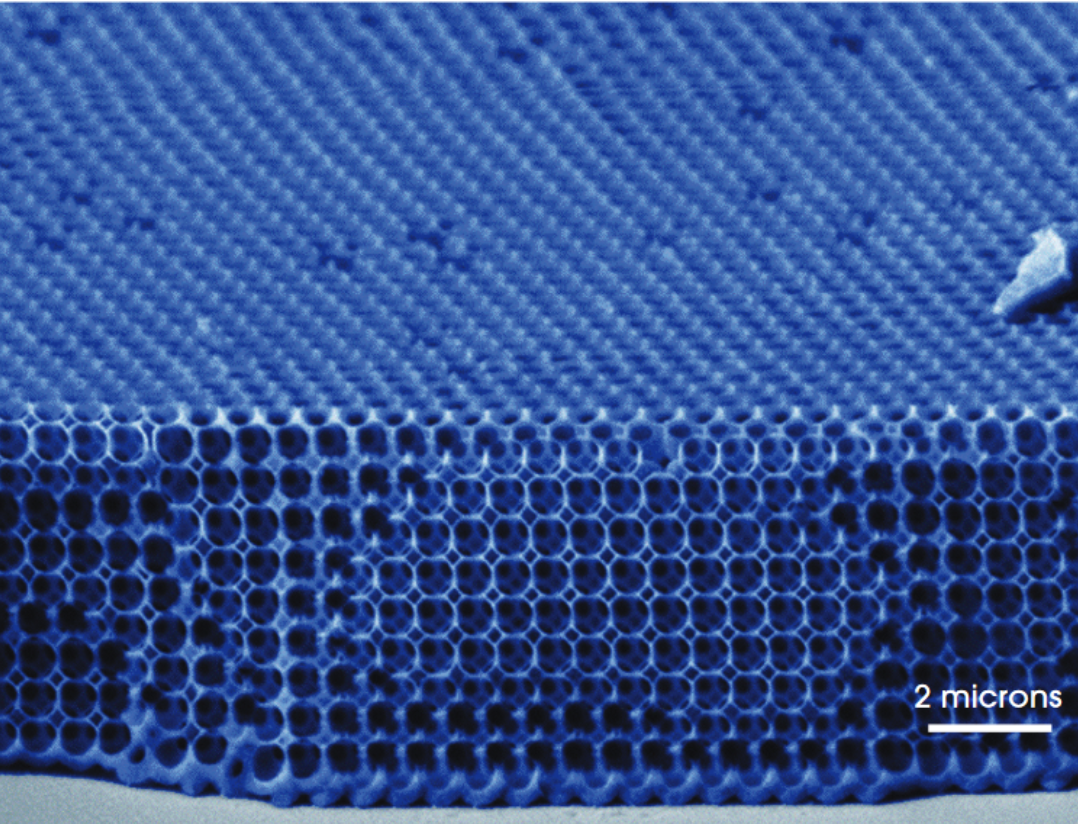
\includegraphics[width=0.6\linewidth]{inv_opals.png}
  \caption{逆オパール構造の電子顕微鏡像 \cite{text} p.103 より引用}
  \label{fig:inverse_opals}

\end{figure}

微細な球体を懸濁させたコロイドを蒸発させることによりfcc格子に自己集合させることができるので合成オパールは容易に製造することができる。合成オパールの球間に高誘電体物質を浸透させ、球を溶解させることで構造を反転させ、空気穴の逆オパールを作製することができる。

\section{ウッドパイル構造}
ウッドパイル構造は、棒状の誘電体物質を直行する方向に交互に積み重ねたものである。誘電体は丸太のような形状もあれば長方形の場合もある。
\begin{figure}[htbp]
  \centering
  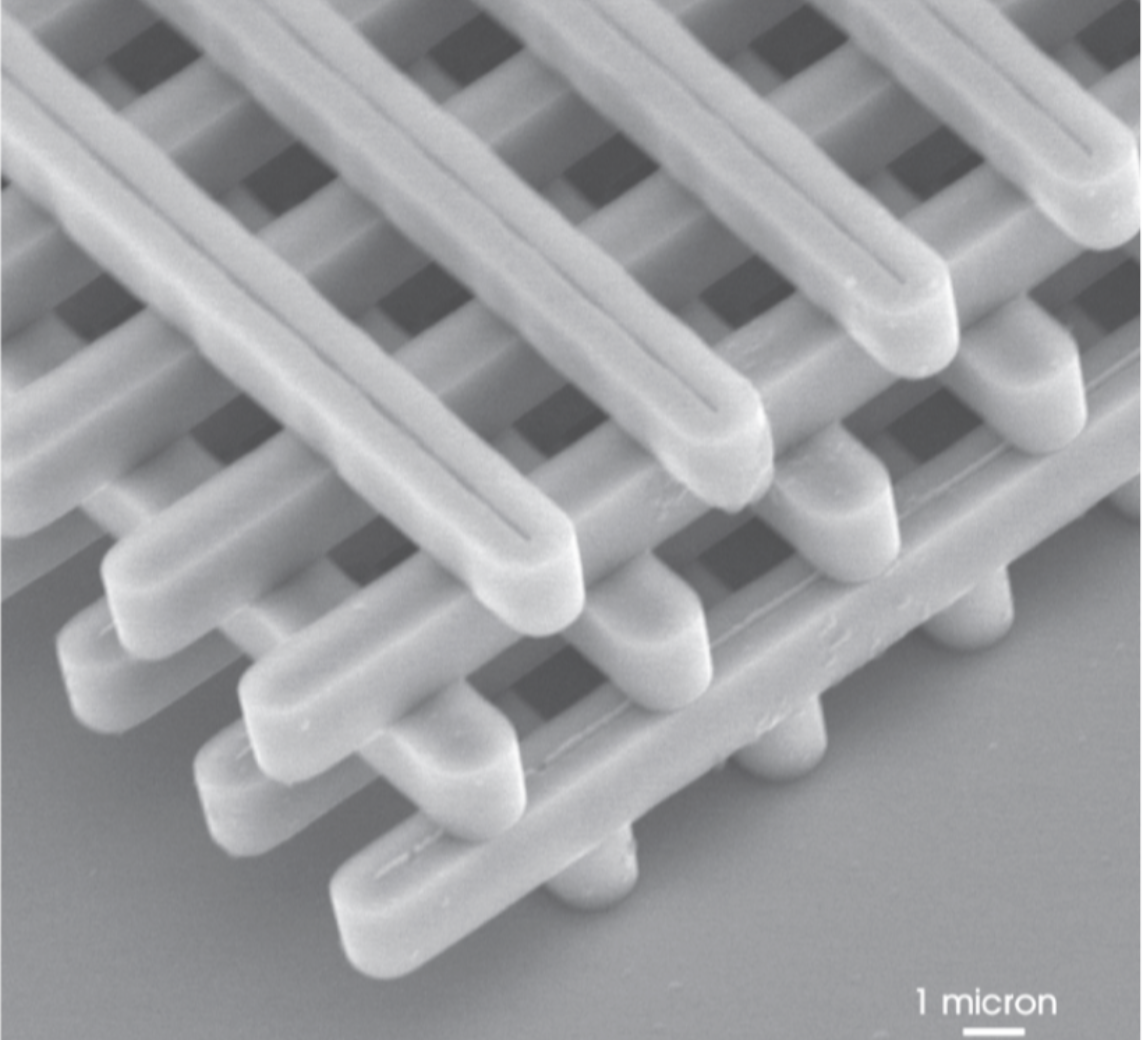
\includegraphics[width=0.6\linewidth]{woodpile.png}
  \caption{ウッドパイルフォトニック結晶の電子顕微鏡像 \cite{text} p.102 より引用}
  \label{fig:woodpile}

\end{figure}
最も単純に直行する方向に交互に積み重ねたものは、図\ref{fig:woodpile}のように、直方体の誘電体を交互に積み重ねたものである。この構造の場合、大きなギャップは生じない。より大きなギャップを生じさせるためには、ある方向を向いた層Aとそれに直交する方向の層Bに対して、それぞれ水平方向に半分だけずらした層C、Dを用いてABCDABCD$\cdots$のように並べることが有効である。

\section{ヤブロノバイト構造}
ヤブロノバイト構造は、図\ref{fig:yablonovite}のような構造をしており、発見者であるEli Yablonovitchらにちなんで名付けられた結晶構造である。誘電体のスラブ(板状の素材)に三角形配列の穴を開け、それぞれの穴を特定の角度で複数回(通常は三回)掘ることによって形成される。

\begin{figure}[htbp]
  \centering
  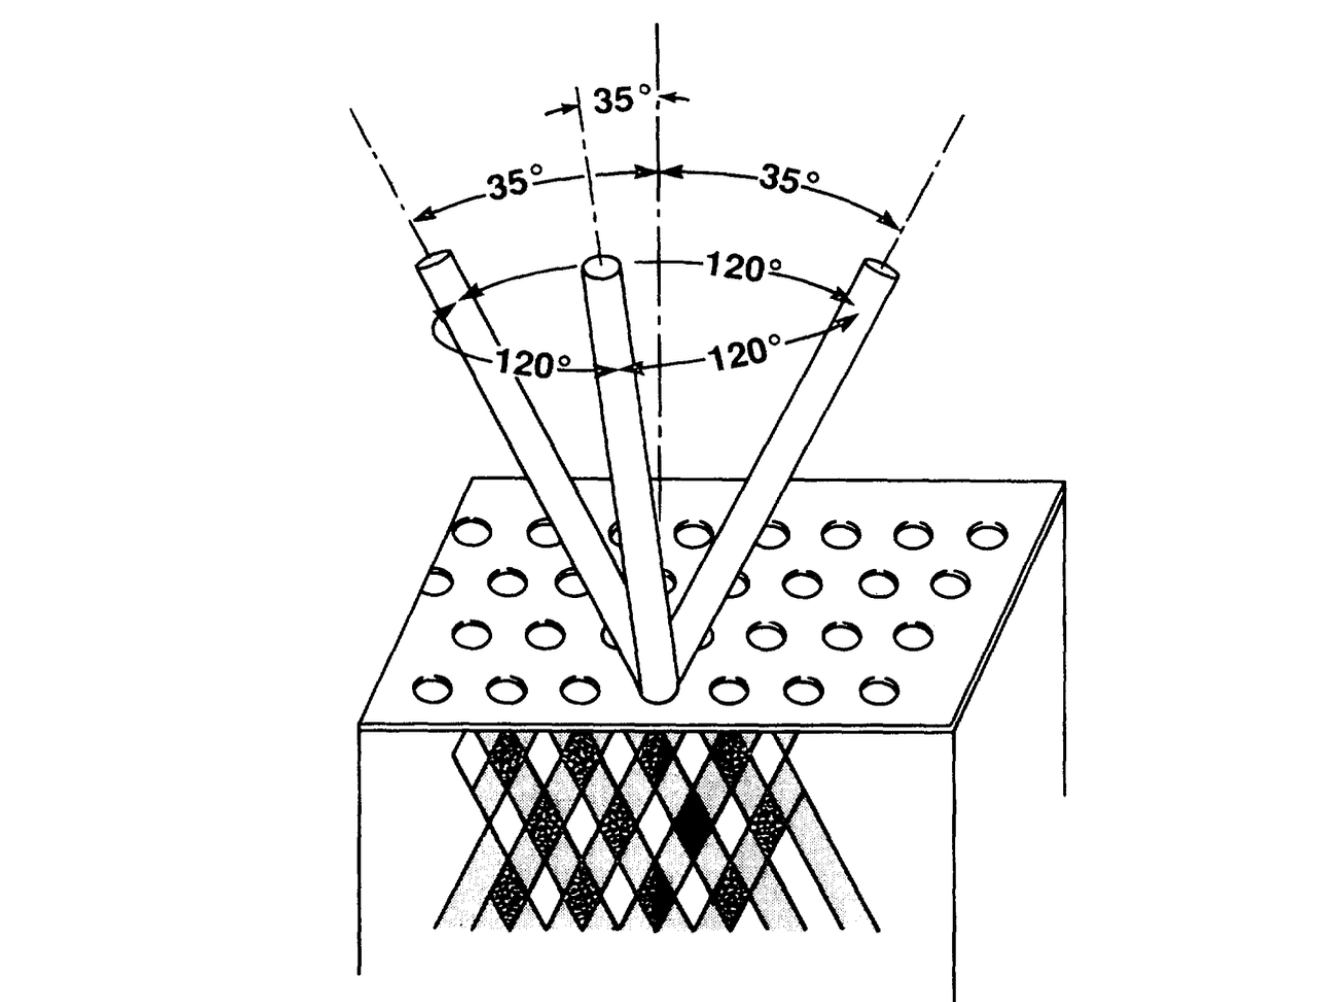
\includegraphics[width=0.6\linewidth]{yablonovite.png}
  \caption{ヤブロノバイト構造 \cite{orig}より引用}
  \label{fig:yablonovite}

\end{figure}


\section{2次元結晶の積み重ね}
\begin{figure}[htbp]
  \centering
  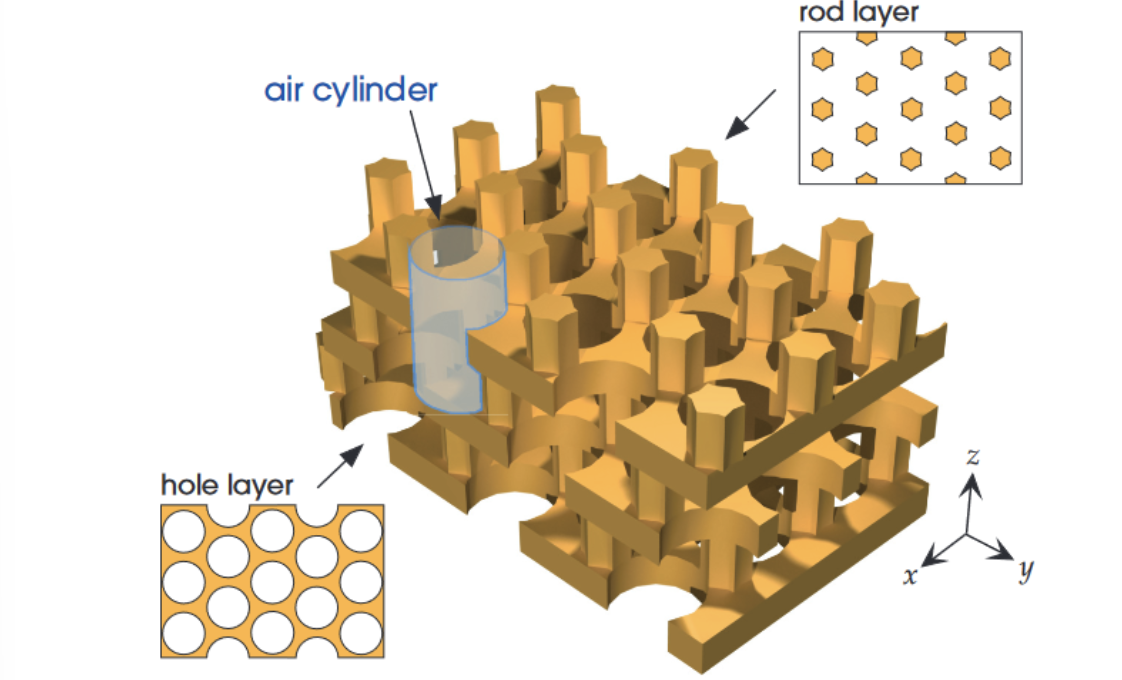
\includegraphics[width=0.6\linewidth]{2d.png}
  \caption{2次元結晶の積み重ねによる3次元結晶の作製 \cite{text} p.106 より引用}
  \label{fig:2d_3d}
\end{figure}
2次元結晶の積み重ねによって3次元結晶を作製することができる。

この結晶は空気中の高誘電体ロッドを三角格子状に並べたロッド層と、高誘電体中に円筒状の空気孔を三角格子状に並べたホール層により構成されている。

\section{ギャップ-ミッドギャップ比}
なぜ評価手法にギャップ-ミッドギャップ比を用いるのかについて述べる

結論:フォトニックバンドギャップの広がりは、その周波数幅$\Delta \omega$で特徴付けることができますが、結晶のスケールに依存してしまう
\end{document}